\documentclass[12pt,oneside,a4paper,parskip=half]{scrbook}

% Sprachanpassung und Grundkonfiguration
\usepackage[utf8]{inputenc}
\usepackage[T1]{fontenc}
\usepackage[ngerman]{babel}
\usepackage{lmodern}
\usepackage{microtype}
\usepackage{csquotes}
\usepackage{hyphenat}
\usepackage{newunicodechar}
\newunicodechar{ }{\,}

% Seitenlayout
\usepackage[a4paper,left=20mm,right=20mm,top=20mm,bottom=25mm]{geometry}
\usepackage{setspace}
\onehalfspacing
\sloppy

% Diagramme
\usepackage{pgfplots}
\pgfplotsset{compat=1.17}

% Mathematik & Symbole
\usepackage{amsmath,amsfonts,amssymb}

% Tabellen & Grafiken
\usepackage{graphicx}
\usepackage{float}
\usepackage{booktabs}
\usepackage{longtable}
\usepackage{tabularx}
\usepackage{pdflscape}
\usepackage{placeins}
\graphicspath{{./}{./figures/}{./assets/}}

% Aufzählungen
\usepackage{enumitem}

% Farben (nur noch für Links oder Basics)
\usepackage{xcolor}

%%%%%%%%%%%%%%%%%%%
%% definitions
%%%%%%%%%%%%%%%%%%%
\def\BaAuthor{Noah Raupold (5022097),\\ David Gläsle (5022114)}
\def\BaAuthorPDF{Noah Raupold (5022097), David Gläsle (5022114)}
\def\BaAuthorStudyProgram{Informatik}
\def\BaType{Internet of Things}
\def\BaTitle{E-Nose}
\def\BaDeadline{\today}

\def\iswithfullname{1}
\ifdefined\iswithfullname
\def\ShowBaAuthor{\BaAuthor}
\else
\def\ShowBaAuthor{N.~N.}
\fi

\newcommand{\TitleGraphic}{
\IfFileExists{logo.png}{

\includegraphics[width=0.5\textwidth]{logo.png}%
}{
\fbox{\parbox[c][3cm][c]{0.5\textwidth}{Logo.png fehlt}}%
}% 
}

\newcommand*{\forcetwosidetitle}{
\begingroup
\cleardoubleoddpage
\KOMAoptions{titlepage=true}%
\csname @twosidetrue\endcsname
\maketitle
\endgroup
}

\newcommand{\TOCbreak}{\\
}

% Bibliografie (Biber)
\usepackage[backend=biber,style=numeric]{biblatex}
\IfFileExists{literatur.bib}{\addbibresource{literatur.bib}}{}

% Hyperlinks
\usepackage{hyperref}
\hypersetup{
colorlinks=true,
linkcolor=black,
filecolor=magenta,
urlcolor=cyan,
pdfauthor={\BaAuthorPDF},
pdftitle={\BaTitle}
}

\begin{document}

%%%%%%%%%%%%%%%%%%%
%% Titelseite
%%%%%%%%%%%%%%%%%%%
\frontmatter
\titlehead{Technische Hochschule Würzburg-Schweinfurt\\Fakultät Informatik und Wirtschaftsinformatik}
\subject{\BaType}
\title{\texorpdfstring{\BaTitle\\[15mm]\TitleGraphic}{\BaTitle}}
\author{\ShowBaAuthor}
\date{\normalsize{Eingereicht am: \BaDeadline}}
\forcetwosidetitle

%%%%%%%%%%%%%%%%%%%
%% Inhaltsverzeichnis
%%%%%%%%%%%%%%%%%%%
\newpage
\setcounter{secnumdepth}{4}
\setcounter{tocdepth}{4}
\tableofcontents

%%%%%%%%%%%%%%%%%%%
%% Main part of the thesis
%%%%%%%%%%%%%%%%%%%
\mainmatter

\chapter*{Kurzfassung}
\addcontentsline{toc}{chapter}{Kurzfassung}

Die vorliegende Projektarbeit befasst sich mit der Konzeption und Implementierung einer elektronischen Nase (\enquote{E-Nose}) zur automatisierten Erkennung faulender Lebensmittel im Kühlschrank. Ziel ist die frühzeitige Detektion von Verderbprozessen durch die Analyse der Umgebungsluft. Das entwickelte System kombiniert präzise Umweltsensorik (CO\textsubscript{2}, Temperatur, Luftfeuchtigkeit) mit einem Metalloxid-Gassensor zur Erfassung flüchtiger organischer Verbindungen (VOCs).

Die erfassten Zeitreihendaten werden in einer InfluxDB-Datenbank zentralisiert und dienen als Trainingsgrundlage für ein Machine-Learning-Modell. Hierbei kommt ein moderner Transformer-basierter Ansatz (Masked Autoencoder) zum Einsatz, der durch selbstüberwachtes Lernen (Self-Supervised Learning) ein Verständnis für die normalen atmosphärischen Zyklen entwickelt. Anomalien, wie sie durch Gärprozesse oder Fäulnis entstehen, können so anhand von Abweichungen in den rekonstruierten Sensordaten identifiziert werden. Als universitäres Projekt fokussiert die Arbeit die Machbarkeit und methodische Evaluierung eines Prototyps und erhebt keinen Anspruch auf eine zertifizierte Lebensmittelsicherheitslösung. Diese Arbeit dokumentiert den Hardware-Aufbau, die Software-Architektur der Datenerfassung sowie die methodischen Grundlagen der verwendeten KI-Modelle.

\chapter{Einleitung}

\section{Motivation}
Lebensmittelverschwendung ist ein globales Problem mit signifikanten ökonomischen und ökologischen Auswirkungen. Ein Großteil des Verderbs im privaten Haushalt geschieht unbemerkt in geschlossenen Lagerorten wie Kühlschränken. Während das menschliche Auge sichtbaren Schimmel erkennen kann, bleiben frühe chemische Anzeichen des Verfalls – wie der Anstieg von CO\textsubscript{2} durch bakterielle Atmung oder die Freisetzung spezifischer Gase – oft lange unbemerkt.

\section{Zielsetzung}
Das primäre Ziel dieses Universitätsprojekts ist die \textbf{frühzeitige Erkennung von Lebensmittelverderb} im Kühlschrank. Im Fokus steht die prototypische Umsetzung und methodische Bewertung. Da Mikroorganismen wie Bakterien und Pilze bereits in frühen Wachstumsphasen Stoffwechselprodukte an die Umgebungsluft abgeben, kann ein sensorgestütztes System den Verfall detektieren, noch bevor dieser visuell oder olfaktorisch für den Menschen wahrnehmbar ist. 

Dabei liegt der Fokus auf zwei Kernaspekten:
\begin{enumerate}
    \item \textbf{Detektion metabolischer Marker:} Erfassung des CO\textsubscript{2}-Anstiegs durch bakterielle Respiration und der Zunahme flüchtiger organischer Verbindungen (VOCs) durch Fermentationsprozesse.
    \item \textbf{Kompensation von Störgrößen:} Da auch menschliche Aktivitäten (Türöffnungen) oder technische Zyklen (Abtauphasen) Sensorwerte beeinflussen, muss das System lernen, zwischen \enquote{normalem} Verhalten und \enquote{biologischen Anomalien} zu unterscheiden.
\end{enumerate}

\chapter{Grundlagen und Technologien}

\section{Sensortechnologie}
Die Detektion von Verderb beruht auf der Überwachung spezifischer chemischer und physikalischer Indikatoren.

\begin{figure}[H]
    \centering
    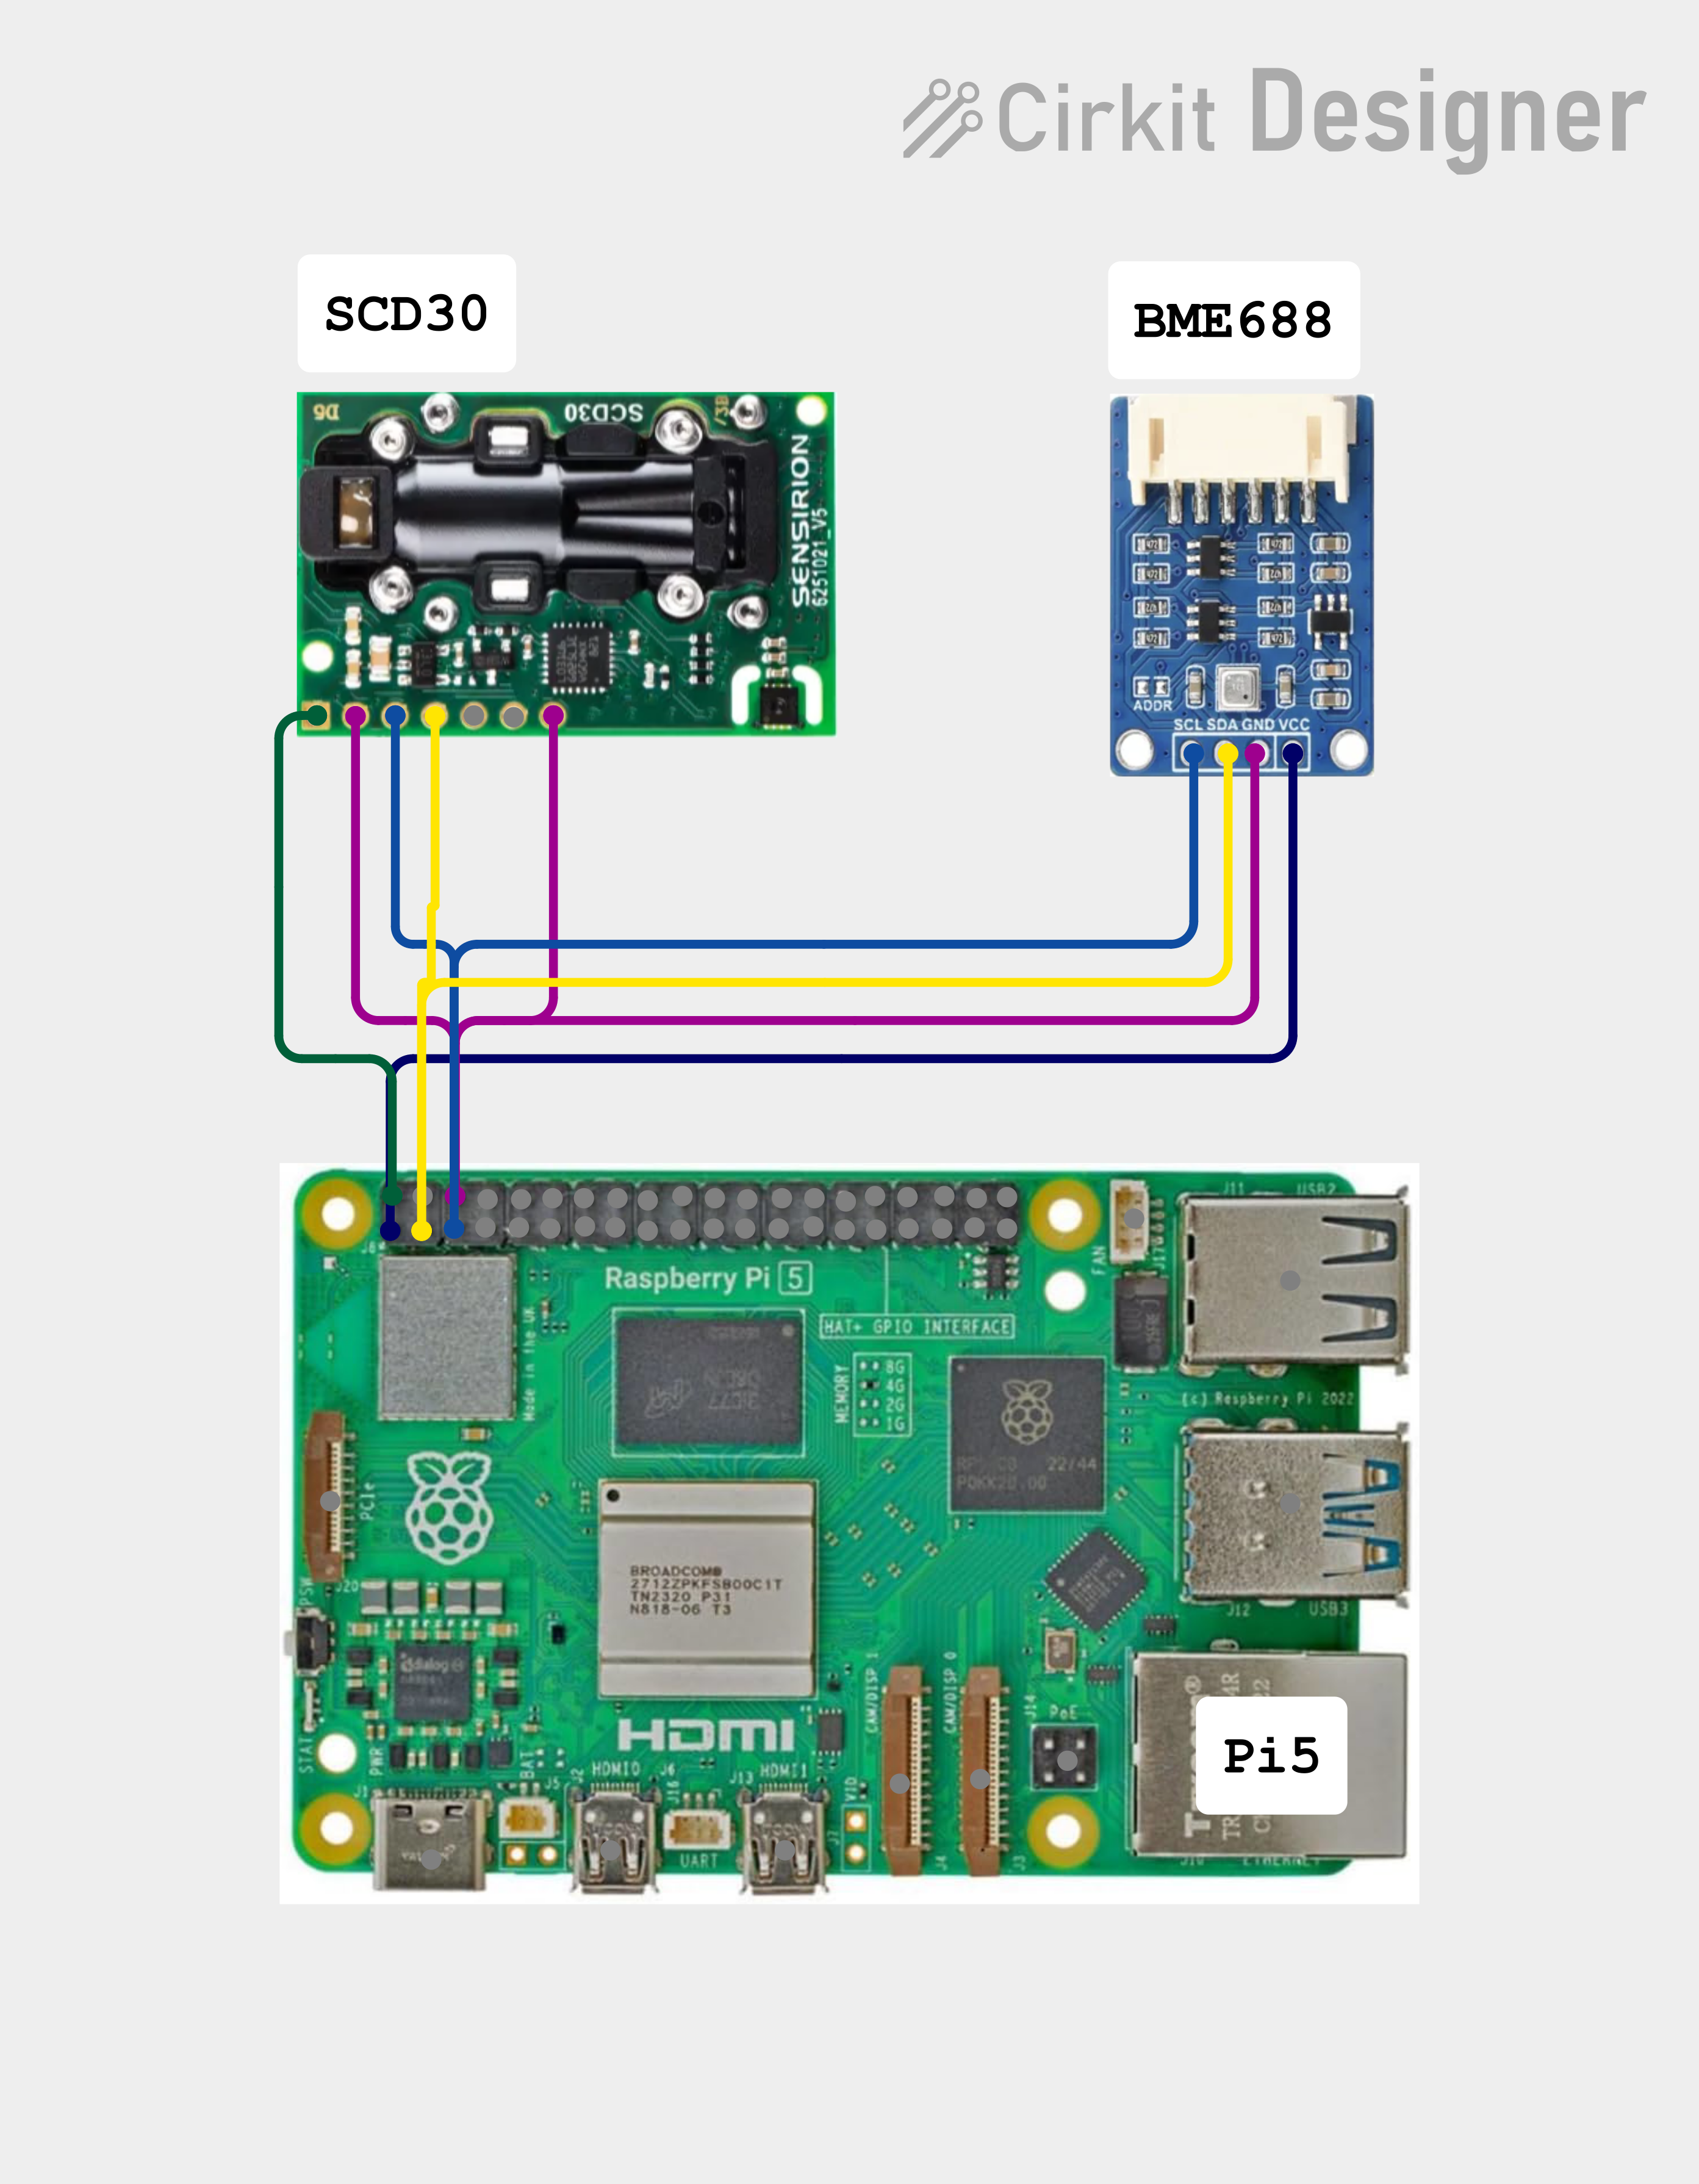
\includegraphics[width=0.6\textwidth]{circuit.png}
    \caption{Schaltplan und I\textsuperscript{2}C-Verkabelung der Sensoren}
\end{figure}

\subsection{SCD30 - NDIR CO\textsubscript{2} Sensor}
Der Sensirion SCD30 nutzt das Prinzip der nicht-dispersiven Infrarotabsorption (NDIR).
\begin{itemize}
    \item \textbf{Biologischer Hintergrund:} Viele aerobe Verderberreger (z.B. Schimmelpilze) produzieren CO\textsubscript{2} als Nebenprodukt ihrer Atmung. In einem geschlossenen Kühlschrank führt dies zu einem messbaren Konzentrationsanstieg über den atmosphärischen Hintergrundwert hinaus.
    \item \textbf{Messprinzip:} CO\textsubscript{2}-Moleküle absorbieren Licht bei 4.3 $\mu$m. Der SCD30 erlaubt eine präzise Bestimmung ohne die Querempfindlichkeiten billigerer elektrochemischer Sensoren.
\end{itemize}

\subsection{BME688 - 4-in-1 Gassensor}
Der Bosch BME688 ist ein Metalloxid-Halbleitersensor (MOX) mit integrierter KI-Unterstützung für VOC-Muster.
\begin{itemize}
    \item \textbf{Biologischer Hintergrund:} Während der Zersetzung von Proteinen und Fetten entstehen flüchtige Verbindungen wie Ethylen, Ethanol, Schwefelwasserstoff oder Ammoniak. Diese bilden den charakteristischen \enquote{Geruch} von Verderb.
    \item \textbf{Messprinzip:} Die Leitfähigkeit der Metalloxidschicht ändert sich bei Kontakt mit diesen reduzierenden Gasen. Der BME688 ist besonders sensitiv gegenüber einem breiten Spektrum dieser biologischen Marker.
\end{itemize}

\section{Software-Architektur}
Das System setzt auf eine modulare Python-Architektur.

\subsection{Asynchrone Datenerfassung}
Um Datenlücken zu vermeiden, arbeitet der Datenlogger asynchron. Die Kommunikation mit der Datenbank (InfluxDB) wird vom Sensor-Ausleseprozess entkoppelt. Dies stellt sicher, dass Netzwerk-Latenzen nicht die Abtastrate der Sensoren (Sampling Rate) beeinträchtigen. Zeitstempel werden mittels \texttt{time.monotonic()} präzise getaktet, um Drift über lange Laufzeiten zu verhindern.

\subsection{InfluxDB}
Als Speicherlösung dient InfluxDB, eine auf Zeitreihen spezialisierte Datenbank (Time Series Database - TSDB). Sie eignet sich ideal für IoT-Daten, da sie hohe Schreibgeschwindigkeiten unterstützt und effiziente Abfragen über Zeitfenster ermöglicht.

\section{Künstliche Intelligenz: Masked Autoencoder}
Zur Anomalieerkennung wird kein klassischer Klassifikator (Gut/Schlecht), sondern ein \textbf{Masked Autoencoder (MAE)} eingesetzt.

\subsection{Funktionsweise}
Ein Autoencoder ist ein neuronales Netz, das lernt, seinen Input zu komprimieren (Encoder) und wiederherzustellen (Decoder). Der \enquote{Masked} Ansatz, bekannt aus Modellen wie BERT oder Vision Transformers, erschwert diese Aufgabe: Teile der Eingabedaten werden zufällig ausgeblendet (\enquote{maskiert}). Das Modell muss lernen, die fehlenden Werte anhand des Kontexts der verbleibenden Sensoren vorherzusagen.

\subsection{Anwendung im Projekt (FridgeMoCA)}
Unser Modell (\enquote{FridgeMoCA}) lernt die normalen physikalischen Zusammenhänge im Kühlschrank (z.B. \enquote{Wenn der Kompressor anspringt, sinkt die Temperatur und die Luftfeuchtigkeit ändert sich}). Kann das Modell die aktuellen Sensorwerte nur mit hohem Fehler rekonstruieren, weicht das aktuelle Geschehen vom gelernten Normalzustand ab – eine Anomalie liegt vor.

%%%%%%%%%%%%%%%%%%%
%% Literatur
%%%%%%%%%%%%%%%%%%%
\backmatter
\nocite{*}
\printbibliography

\end{document}
